\lstdefinestyle{ubuntu}
{
    backgroundcolor=\color{black},
    basicstyle=\scriptsize\color{green}%\ttfamily
}

This appendix ought to give concrete knowledge to utilize the \gls{ros} environment wrt. the \gls{daVinci} surgery robot at Aalborg University as it comprises an immense load of files, packages and various GUI interfaces. It also intends to provide an overview of the code structure and the underlying thoughts. The \gls{ros} environment is currently only developed for Ubuntu. The content of this appendix is accordingly assuming Ubuntu as operating system and assumes additionally basic knowledge in Unix. 

To install ROS on a private laptop, it is recommended to follow the below URL:

\hspace{1cm} {\color{blue}{\textit{http://wiki.ros.org/ROS/Installation}}}

Once ROS is installed, it is possible to work on the \texttt{surgery-srv.lab.es.aau.dk} computer. It may introduce some advantages to work directly on the server in the lab as it provides additional GUI applications such as rviz, but it is obviously more convenient to work from a private laptop and the GUIs can be set-up without too much trouble. Connection to the server can be established through \texttt{ssh}:

%\begin{lstlisting}[style=ubuntu]
\hspace{1cm} \texttt{\$ ssh <user>@surgery-srv.lab.es.aau.dk}
%\end{lstlisting}

To get started with everything, open a terminal and initialize a ROS workspace as:

\hspace{1cm} \texttt{\$ mkdir -p daVinci\_ws/src}

Then navigate to the source directory (\texttt{src}) and type:

\hspace{1cm} \texttt{\$ catkin\_init\_workspace}

This creates a number of necessary files and folders. The code located at the "Robotic Surgery Group - Aalborg University" can be copied/cloned to the \texttt{src} folder. %({\color{blue}{\textit{https://github.com/AalborgUniversity-RoboticSurgeryGroup/}}}).
The original environment (clean configuration) can e.g. be cloned with the following git terminal commands:\vspace{0.1cm}

\hspace{0cm} \texttt{\$ git clone https://github.com/AalborgUniversity-RoboticSurgeryGroup/davinci\_description}

\hspace{0cm} \texttt{\$ git clone https://github.com/AalborgUniversity-RoboticSurgeryGroup/davinci\_driver}

%\hspace{0cm} \texttt{\$ git clone https://github.com/AalborgUniversity-RoboticSurgeryGroup/davinci\_moveit\_config}\vspace{0.2cm}

Each command copies a package. The name and file structure of a package should follow a certain standard, i.e. the \gls{rep} (it is not just the packages which should follow the \gls{rep} standard, but in fact the entire ROS workspace). This ought to make it easier to share and reuse code. The code developed in this thesis obeys to a large extend the \gls{rep}s but exceptions may occur. 

The two initial packages used are in that sense:
\begin{itemize}
\item \texttt{davinci\_description}
\item \texttt{davinci\_driver}
%\item \texttt{davinci\_moveit\_config}
\end{itemize}
If the installation takes place on a local laptop, be sure to install all ROS dependencies. The necessary dependencies can be checked by running \texttt{rosdep check <package\_name>}.

To build the entire environment, open a terminal, navigate to the root of the workspace (\texttt{daVinci\_ws/}) and type:

\hspace{1cm} \texttt{\$ catkin\_make}

This connects all executables and the environment should hereafter be ready for use.
\section{General structure of a ROS setup}
After the workspace is created (called \texttt{daVinci\_ws}), the packages are cloned and the environment is build, the overall code structure should look like the tree structure found below:

\vspace{0.5cm}

\begin{tikzpicture}[scale=1]
\Tree [.\color{blue}{\texttt{daVinci\_ws}}
  [.\color{blue}{\texttt{build}} \text{make files etc.} ]  [.\color{blue}{\texttt{devel}} lib/setup ]  
     [.\color{blue}{\texttt{src}} {\color{white}{m}}$\underset{\text{input to the CMake build system}}{\text{\color{ForestGreen}{\texttt{CMakeLists.txt}}}}${\color{white}{m}} [.\hspace{0.2cm}\text{package $1$}\hspace{0.2cm} $\cdots$ $\cdots$ ]
     [.\hspace{0.2cm}\text{package 2}\hspace{0.2cm} $\cdots$ $\cdots$ ] \hspace{0.2cm}$\cdots$\hspace{0.2cm}  [.\hspace{0.2cm}\text{package $n$}\hspace{0.2cm} $\cdots$ $\cdots$  ]   ] 
  ]
\end{tikzpicture}
  
\vspace{0.2cm}

Each package has a similar structure. While the content of each package may vary, they always have a file called \texttt{package.xml} and \texttt{CMakeLists.txt}, and often the structure shown below.

%\begin{tikzpicture}[scale=1]
\hspace{2.5cm}
\Tree [.\text{package $m$} \color{ForestGreen}{\texttt{CMakeLists.txt}} \color{ForestGreen}{\texttt{package.xml}} [.\color{blue}{\texttt{config}} $\cdots$ $\cdots$ ]  [.\color{blue}{\texttt{launch}} $\cdots$ $\cdots$  ] [.\color{blue}{\texttt{others}} $\cdots$ $\cdots$ ] $\cdots$ ]
%\end{tikzpicture}



%%%>
\begin{comment}
:Title: Simple graph
:Tags: Arrows;Diagrams;Graphs;Mathematics
:Author: Stefan Kottwitz
:Slug: graph

A simple example of a graph with straight and bend arrows and loops.
It has been posted as answer to the question
http://tex.stackexchange.com/q/45734/213 of Ichibann.

* Define styles for edges, arrows, and nodes
* Place the main nodes
* Draw edges with nodes for description
* Use options `loop` and `bend` for loops and bent edges
* Specify `left` and `right` for bend direction and node placement
\end{comment}

Before elaborating on the significance of these folders and files, it is to some extend important to have an overview of the general used terms in the \gls{ros} environment. Those terms are briefly mentioned in \autoref{ros:node_etc}. 
\begin{figure}[H]
\center
\begin{tikzpicture}[->,>=stealth',shorten >=1pt,auto,node distance=5.5cm,
  thick,main node/.style={circle,fill=blue!20,draw,font=\sffamily\Large\bfseries}]
  \node[main node] (1) {\small \text{rosnode 1}};
  \node[main node] (2) [right of=1] {\small \text{rosnode 2}};

  \path[every node/.style={font=\sffamily\small}]
    (1) 
         edge node [right] {\hspace{-1.3cm}$\overset{\text{\normalsize rostopic}}{\text{\color{black}{(communication)}}}$} (2)
      %  edge [bend right] node[left] {0.3} (2)
      %  edge [loop above] node {0.1} (1)
      %  edge [bend right] node[right] {0.2} (2)
    (2) %edge node [right] {} (1)
        %edge [loop right] node {0.6} (2)
        %edge [bend right] node[right] {0.2} (1)
        ;
\end{tikzpicture}
\caption{Coherence between rosnodes and rostopics. A node is simply a process that performs some computation/algorithm and a topic is the communication channel between two or more ROS nodes. Two often used terms in this context are to publish/subscribe to a topic. To "publish" means to send a message from a topic and one can decode the message by "subscribing" to a topic.}
\label{ros:node_etc}
\end{figure}
With a basic understanding of ROS nodes and topics, the generic content of the two required files (\texttt{CMakeLists.txt} and \texttt{package.xml}) and the often used \texttt{launch} folder can be elaborated in \autoref{tab:eleb}. Other folders and files like \texttt{src}, \texttt{config}, \texttt{include} and similar are indeed also often used. They all have the purpose to enhance overview. The name should to some extend be self explaining, e.g. the \texttt{config} folder includes configuration files for the da-Vinci robot, the \texttt{src} folder often includes C++ files used for algorithms designed for specific purposes etc.
\begin{table}[H]
\begin{tabularx}{\textwidth}{X X X}
\rowcolor{HeaderBlue} 
 \textbf{\texttt{CMakeLists.txt}} & \textbf{\texttt{package.xml}}& \textbf{launch} \\
Package/project description, \gls{catkin} version, specification of required packages (not ROS packages but packages to create CMake environment variables), catkin dependencies and definitions and the specification of catkin build targets (executables and library targets). 
%%
$^*$  & Also referenced as a package manifest. It provides information about the maintainer, version, package name (e.g. \texttt{davinci\_driver}) and author. It specifies build tool dependencies (for the package to build itself - typically only catkin), build dependencies (required packages at build time), run-time dependencies and test dependencies (not used).  $^{**}$ & The content of a launch folder is primary used to start a group of nodes with unique topics and/or parameters. They are executed by the \texttt{roslaunch} terminal command followed by package name and lastly the name of the launch file, i.e.:\newline \texttt{roslaunch <package name> <name of launch file>}. \\  \rowcolor{textBlue}
\end{tabularx}
	\caption{Brief explanation of the purpose of the most common used folder names in a package.\newline $^*$ \citep{bib:CmakeLists}, $^{**}$ \citep{bib:package}.} 
\label{tab:eleb}
\end{table}
\vspace{-0.2cm}
With a somewhat superficial, but sufficient, introduction to \gls{ros}, the concrete interfacing can be considered.
\vspace{-0.4cm}
\section{Setup of Low Level Control and how to Initiate ROS}\label{sec:init_ROS}
\vspace{-0.2cm}
Before the communication between ROS and da Vinci may be considered, all low level PID controllers must run correctly and the RIO configuration must be performed. 

From the \texttt{aau86730} computer, launch the \texttt{p4\_primary\_Control} icon located on the desktop and connect \texttt{RT Single Board RIO (172.26.12.32)} by right clicking the icon and press connect. Subsequently, navigate to \texttt{p4\_prim\_control\_FPGA\_multichannel\_7\_FLOAT\_SPI\_5.vi} and open it. This launch a GUI comprising access to the seven low level controllers which are activated from the arrow in the upper left corner. The controller gains, setpoints, maximum step size and various calibration options are easily accessible from this GUI, though it should not be necessary to modify any of those. 

Be sure that the gearing factors are specified as follows:
\begin{table}[H]
\begin{tabularx}{\textwidth}{X X X X X X X}
\rowcolor{HeaderBlue} 
\scriptsize \textbf{Intrument Jaw Left} &\scriptsize  \textbf{Intrument Jaw Right} &\scriptsize  \textbf{Intrument Pitch} &\scriptsize  \textbf{Instrument Roll} &\scriptsize  \textbf{Instrument Slide} & \scriptsize   \textbf{Hand Pitch} &  \scriptsize\textbf{Hand Roll}\\
12 & 12 & 12.4 & 7.5 & 1340 & 200 & 200\\
\end{tabularx}
	\caption{Measured gearing factors. Gearing factors are measured such that $\pi$/4 from \gls{ros} corresponds to 45 degrees on the real robot.}
\label{tab:gearing}
\end{table}
To allow the ROS environment access to the full range of setpoints, launch \texttt{p4-control\_prim-main4.vi} and activate this GUI in a similar manner. This GUI acts merely as interface and offers no user options as such. All necessary setup before initiating ROS is at this point in time performed.
\subsubsection*{ROS}
It is important to notice that every time a new terminal is commenced it is important to source the bash file from the workspace, i.e.:

\hspace{1cm} \texttt{\$ source devel/setup.bash}

The following list of commands must be executed from the root of the workspace. It is first of all important to collect all \gls{node}s such that they are able to communicate with each other. Open a terminal and run:

\hspace{1cm} \textbf{1.} \ \ \ \texttt{\$ roscore} \ \ \ {\color{RoyalBlue}{\textit{\# Leave this running in the terminal}}}

Now, to secure the TCP/IP connection between ROS and the RIO board (Rx \& Tx of setpoints), launch the driver from a new terminal:

\hspace{1cm} \textbf{2.} \ \ \  \texttt{\$ roslaunch davinci\_driver davinci\_driver.launch} \ \ \ {\color{RoyalBlue}{\textit{\# Leave this running}}} 

With these files processes running, the environment is proper set up. The remainder of this appendix will first elaborate what the moveit \gls{api} consist of, why it could be a good idea to use it and why it essentially is not used.
\section{Structure of Moveit and Why it is Not Used}
Moveit is an interface to standard robots. The use of Moveit ought to ease trajectory planning and to ease interfacing with Da Vinci. The moveit package includes the very handy \texttt{move\_group} node which searches for a \gls{urdf} which is a description of the robot (containing parameters like joint limits, kinematics etc.) and it searches for a \gls{srdf} which is 	a parameter generated by the setup assistant (elaborated in \autoref{app:setup_assist}), thus representing parameters not in the \gls{urdf}. This could be group state configurations or alike.

In that sense the \texttt{move\_group} node offers a (when the ROS learning curve is conquered) sorely easy user interface from both python, C++ and a GUI. It is indeed an apparent starting interface to use, and the first successful interface to the robot was indeed established through the \texttt{move\_group} node and for that reason described in this appendix. As is shall be seen, \texttt{move\_group} has some disadvantages when the objective is a real-time safety controller, which mostly consist of:
\begin{itemize}
\item Speed. The \texttt{move\_group} node offers many features, including static obstacle avoidance and trajectory planning. All very useful applications, but they slow down the process and proofs itself useless when the controllers developed in \autoref{chap:cbf_1d_static} and \autoref{chap:cbf_1d_dynamic} are to be implemented.
\item The \texttt{move\_group} node already includes controllers hence shattering the dynamics modelled. The safety controllers developed are at a lower abstraction layer.
\end{itemize}
A significant amount of code is developed with the \texttt{move\_group} node. The low level details will, however, not be elaborated. However, the results of the work undertaken with the Moveit package, can be cloned as the development branch at github:

\hspace{0cm} \texttt{\$ git clone https://github.com/AalborgUniversity-RoboticSurgeryGroup/davinci\_moveit\_config ---branch develop} \ \ \ {\color{RoyalBlue}{\textit{\# Clone both driver, description and Moveit package from the development branch}}}

To give an overview of the code structure when the Moveit package is used, the directory tree on the following page is provided. It shows merely the "interesting files" seen from a developers point of view. In reality, additionally files are present. 
\newpage
\renewcommand*\DTstylecomment{\rmfamily\color{gray}\textsc}
\renewcommand*\DTstyle{\ttfamily\textcolor{blue}}

\begin{figure}[H]
% to make comment:
% .4 davinci\_moveit\_config\DTcomment{Guillaume}.
\dirtree{%
.1 /...
.2 davinci\_ws. %\DTcomment{workspace folder, created by mkdir}.
.3 build. %\DTcomment{generated by catkin\_init\_workspace}.
%.4 \color{gray}{..}.
.4 \color{gray}{... all make-files}. %\DTcomment{generated by catkin\_init\_workspace}.
.3 devel. %\DTcomment{generated by catkin\_init\_workspace}.
%.4 \color{gray}{..}.
.4 \color{gray}{... all libraries and setup files}. %\DTcomment{generated by catkin\_init\_workspace}.
.3 src.
.4 \color{ForestGreen}{CMakeLists.txt}.
.4 davinci\_description. %\DTcomment{\underline{Package:} Physical sizes and rotation matrices}.
.5 \color{ForestGreen}{CMakeLists.txt}.
.5 config.
.6 \color{ForestGreen}{davinci.rviz}.
.5 launch.
.6 \color{ForestGreen}{demo.launch}.
.6 \color{ForestGreen}{visualize\_in\_rviz.launch}.
.5 meshes.
.6 \color{gray}{... all .stl files (used for the 3D model in rviz)}.
.5 \color{ForestGreen}{package.xml}.
.5 robots.
.6 \color{ForestGreen}{remote\_center\_manipulator.xacro}\hspace{0.2cm}\color{gray}{\# rotation matrices for the hand}.
.6 \color{ForestGreen}{davinci.xacro}\hspace{0.2cm}\color{gray}{\# assembles all xml macros}.
.6 \color{ForestGreen}{p4\_arm.xacro}\hspace{0.2cm}\color{gray}{\# rotation matrices for the arm}.
.6 instruments.
.7 \color{ForestGreen}{needle\_driver.xacro}\hspace{0.2cm}\color{gray}{\# rotation matrices for instrument}.
.6 \color{gray}{... + other xacro files}.
.4 davinci\_driver. %\DTcomment{\underline{Package:} Interface with the physical robot}.
.5 \color{ForestGreen}{CMakeLists.txt}.
.5 \color{ForestGreen}{dstp.json}.
.5 launch.
.5 src.  
.6 \color{ForestGreen}{davinci\_driver.cpp}\hspace{0.2cm}\color{gray}{\# establish connection }.
.6 \color{ForestGreen}{ros\_driver.cpp}\hspace{0.2cm}\color{gray}{\# establish connection }.
.6 \color{ForestGreen}{sbrio\_driver.cpp}\hspace{0.2cm}\color{gray}{\# establish connection }.
.5 srv.
.6 \color{gray}{... various hard-coded names}.
.5 config.
.6 \color{ForestGreen}{davinci\_ip\_adresses.yaml}\hspace{0.2cm}\color{gray}{\# set IP for RIO primary/secondary board}.
.6 \color{ForestGreen}{p4\_hand\_controller.yaml}\hspace{0.2cm}\color{gray}{\# specify each controllable joint}.
.5 include.
.6 \color{gray}{... header files for davinci\_driver.cpp and sbrio\_driver.cpp}.
.5 libsjon.
.6 \color{gray}{... various libraries}.
.4 davinci\_moveit\_config. %\DTcomment{\underline{Package:} Trajectory planning}.
.5 \color{ForestGreen}{CMakeLists.txt}.
.5 config.
.6 \color{ForestGreen}{controllers.yaml}\hspace{0.2cm}\color{gray}{\# specifies each controllable joint}.
.6 \color{ForestGreen}{davinci.srdf}\hspace{0.2cm}\color{gray}{\# collision and group specification}.
.6 \color{ForestGreen}{fake\_controllers.yaml}\hspace{0.2cm}\color{gray}{\# simulation controller specification}.
.6 \color{ForestGreen}{joint\_limits.yaml}\hspace{0.2cm}\color{gray}{\# Acceleration, velocity and position limits}.
.6 \color{ForestGreen}{kinematics.yaml}\hspace{0.2cm}\color{gray}{\# Kinematic solver specification}.
.6 \color{ForestGreen}{ompl\_planning.yaml}\hspace{0.2cm}\color{gray}{\# path planning specification}. 	
.5 launch.
.6 \color{ForestGreen}{davinci\_moveit\_controller\_manager.launch.xml}\hspace{0.2cm}\color{gray}{}.
.6 \color{ForestGreen}{move\_group.launch}\hspace{0.2cm}\color{gray}{\# launch all essential drivers }.
.6 \color{ForestGreen}{setup\_assistant.launch}\hspace{0.2cm}\color{gray}{\# launch to generate essential moveit files}.
.6 \color{gray}{... + other launch files controlled by the setup assistant}.
.5 \color{ForestGreen}{package.xml}\hspace{0.2cm}\color{gray}{\# specification of moveit dependencies}.
.5 src.
.6 \color{ForestGreen}{MoveGroupInterface.cpp}\hspace{0.2cm}\color{gray}{\# main C++ interface for Moveit}.
}
%\caption{Code structure in the ROS environment}
\end{figure}
To run the code, be sure that step \textbf{1} and \textbf{2} in \autoref{sec:init_ROS} is carried through. Thus, it is possible to allow trajectory planning, by linking the OMPL (Open Motion Planning Library) to the system by running: 

\hspace{1cm} \textbf{3.a} \ \ \  \texttt{\$ roslaunch davinci\_moveit\_config move\_group.launch} \ \ \ {\color{RoyalBlue}{\textit{\# Leave this running}}} 

If a 3D GUI interface is desired, open a new terminal and launch:

\hspace{1cm} \textbf{3.b} \ \ \  \texttt{\$ roslaunch davinci\_bringup visualization.launch} \ \ \ {\color{RoyalBlue}{\textit{\# This opens rviz}}} 

Press the "add" button in \texttt{rviz} and add the "MotionPlanning" option to the panel where start and goal state can be specified. Hereafter, plan and execute the specified goal. This cause the arm of da Vinci to reach out for the specified goal state consisting of five joint angles.

To launch the developed C++ interface, which allows 3D setpoints (by the KDL inverse kinematic solver) and custom joint specification, open a terminal and type:

\hspace{1cm} \textbf{4} \ \ \  \texttt{\$ rosrun davinci\_moveit\_config MoveGroupInterfaceExecute} \ \ \ {\color{RoyalBlue}{\textit{}}} 

This executes a GUI which provides the following options:

\lstdefinestyle{DOS}
{
    backgroundcolor=\color{white},
    basicstyle=\scriptsize\color{black}\ttfamily
}
\begin{lstlisting}[style=DOS]
*********************************
_________________________________
Press 'j' to specify joint angles
Press 'x' to specify cartesian positions (IK)
Press 'd' to run demo mode
Press 't' to run test mode
Press 'i' to run IK test 
Press 'f' to run FK test 
*********************************
\end{lstlisting}
The \gls{ik} test and \gls{fk} test are executed. Both of them ask the slide position to move to the position 0.05\,cm and move back to 0.00\,cm immediately. Thus no delay between the two queries are desired. The position is concurrently recorded (the recording can be done similar to the setup described in \autoref{app:meas}). Thus the trajectories are plotted in \autoref{fig:moveit_traj}.
\begin{figure}[H]
\centering
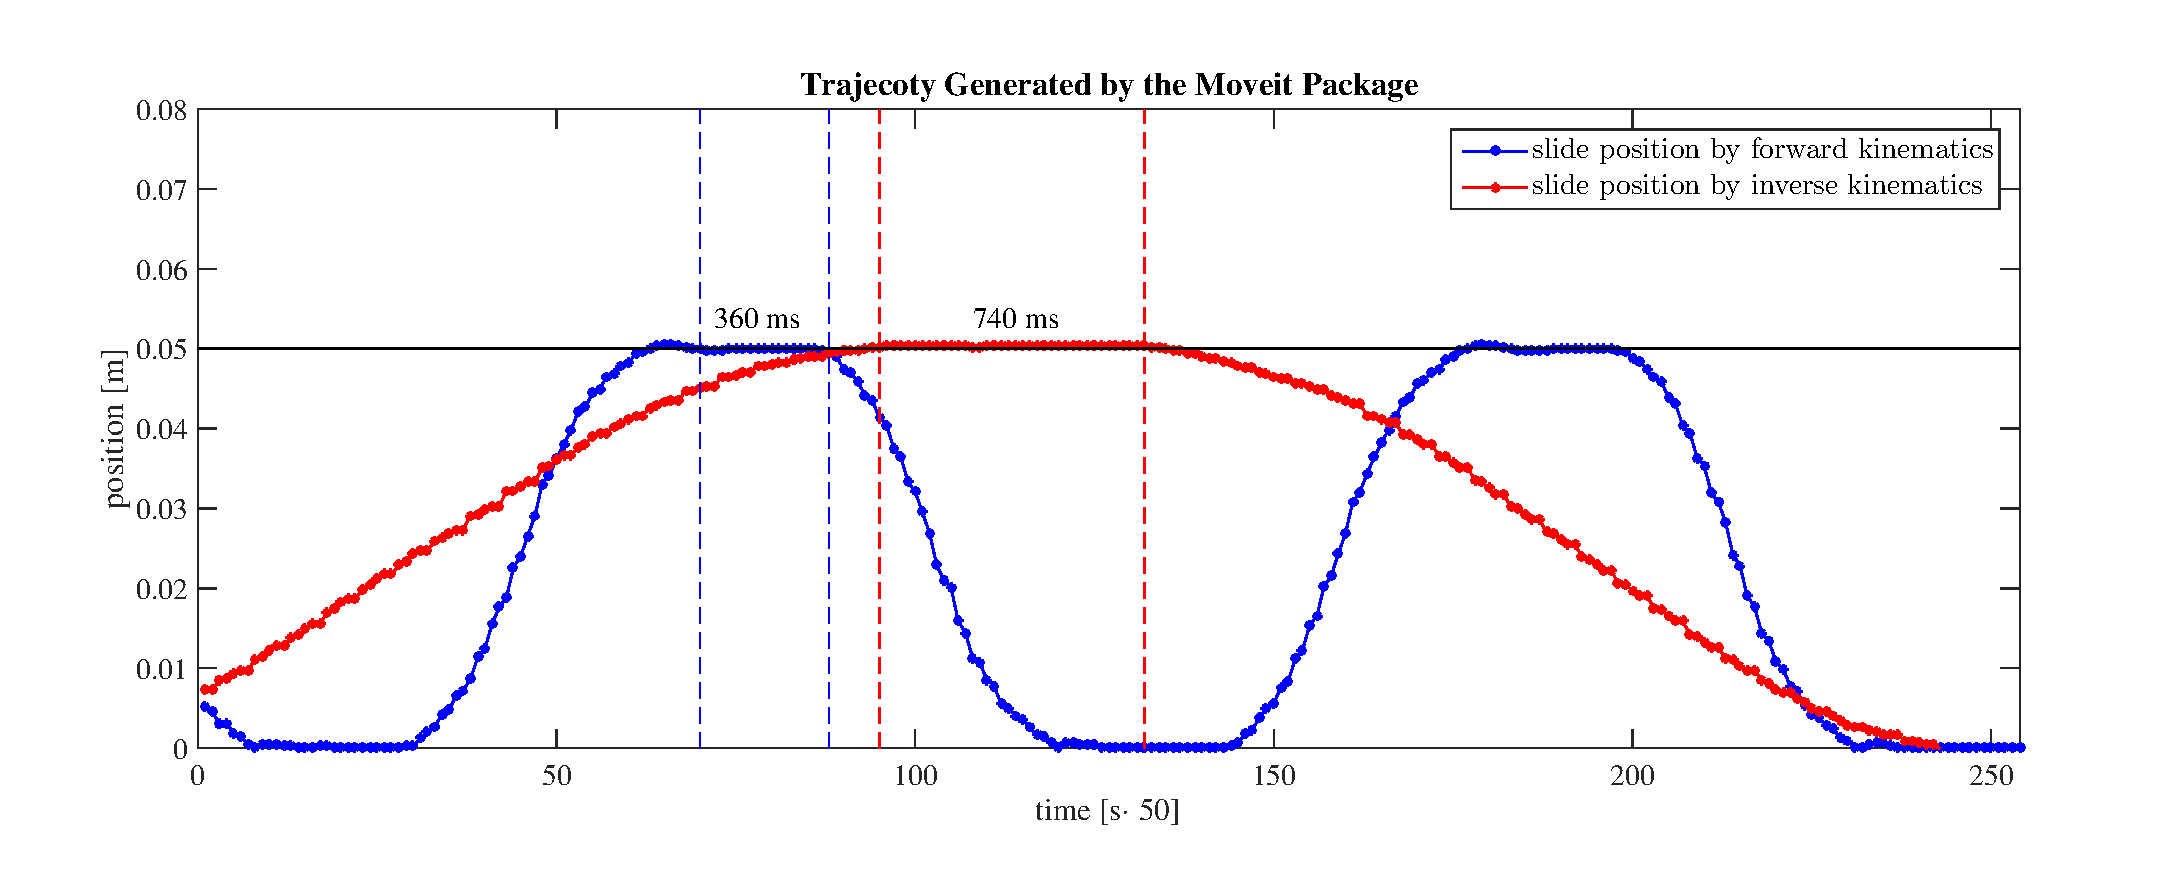
\includegraphics[width=1\textwidth]{traj_moveit.eps}
	\caption{Trajectories plotted by means of Moveit. It is seen that the processing time is high and nearly useless when the objective differs from trajectory planning. The code used to generate the trajectories is showed in \autoref{fig:code-eks-moveit}. It is also seen that the dynamics are limited. Measurement files and plotting details can be found in \autoref{app:cd} by running \texttt{run\_moveit\_trajectory.m} under the path \texttt{measurements/moveit\_test}.}
	\label{fig:moveit_traj}
\end{figure}
As seen from \autoref{fig:moveit_traj}, the \texttt{move\_group} node requires processing time to calculate a trajectory which is nearly useless for real-time controllers. The processing time is due to the highly advanced trajectory generation calculated by the \texttt{move\_group} node. An example of how to use of the \texttt{move\_group} node is provide in \autoref{fig:code-eks-moveit}. The code snippet to the left shows the use of forward kinematics and the code snippet to the right shows how to use the inverse kinematics and it is indeed these code snippets that have been used to generated the trajectories in \autoref{fig:moveit_traj}. It is important to include the proper Moveit libraries and structure of \texttt{CMakeLists.txt} and \texttt{package.xml} correctly. These are found at github when the development branch just described is cloned.
\begin{figure}[H]
    \centering
    \begin{minipage}{.5\textwidth}
\begin{lstlisting}[language=gedit]
while(1) {
      ROS_INFO("set test angles");
      joints[p[2]] =  0;  // hand roll
      joints[p[1]] =  0; // hand pitch
      joints[p[0]] =  0.0; // slide
      joints[p[3]] =  0; // inst roll
      joints[p[4]] =  0; // inst pitch
      joints[p[5]] =  0; // jaw right
      group.setJointValueTarget(joints);
      group.move();

      ROS_INFO("set test angles");
      joints[p[2]] =  0;  // hand roll
      joints[p[1]] =  0; // hand pitch
      joints[p[0]] =  0.05; // slide
      joints[p[3]] =  0; // inst roll
      joints[p[4]] =  0; // inst pitch
      joints[p[5]] =  0; // jaw right
      group.setJointValueTarget(joints);
      group.move();
}
\end{lstlisting}
    \end{minipage}%
    \begin{minipage}{0.5\textwidth}
\begin{lstlisting}[language=gedit]
while(1) {
        geometry_msgs::Pose target_pose3;
        target_pose3.position.x = 0.000000 + off_x;
        target_pose3.position.y = 0.000000 + off_y;
        target_pose3.position.z = 0.050000 + off_z;
        group.setPoseTarget(target_pose3);
        moveit::planning_interface::MoveGroup::Plan my_plan_3;
        bool success_3 = group.plan(my_plan_3);
        ROS_INFO("success = %d", success_3);
        group.move();

        geometry_msgs::Pose target_pose4;
        target_pose4.position.x = 0.000000 + off_x;
        target_pose4.position.y = 0.000000 + off_y;
        target_pose4.position.z = 0.000000 + off_z;
        group.setPoseTarget(target_pose4);
        moveit::planning_interface::MoveGroup::Plan my_plan_4;
        bool success_4 = group.plan(my_plan_4);
        ROS_INFO("success = %d", success_4);
        group.move();
}
\end{lstlisting}
    \end{minipage}
    \caption{The code snippet to the left shows how to use forward kinematics with the \texttt{move\_group} node (\texttt{p} is a string array containing the six joints). The snippet to the right shows how to use the inverse kinematics solver with the \texttt{move\_group} node.}\label{fig:code-eks-moveit}
\end{figure}
The Setup Assistant is an important GUI when the Movit package is used and for that reason described in the upcoming subsection.
\subsection{Setup Assistant}\label{app:setup_assist}
To run the setup assistant, open a terminal, navigate to the root of the workspace and type:

\hspace{1cm} \textbf{$\bullet$} \ \ \  \texttt{\$ roslaunch davinci\_moveit\_config setup\_assistant.launch} \ \ \ {\color{RoyalBlue}{\textit{\# GUI is launched}}} 

A GUI offering eight setup options will now be present. Load the current \texttt{davinci\_moveit\_config} package. The content of the eight options will be explained in the below itemize as it is important that all options are configured correctly for the kinematic solver to work correctly.
\begin{enumerate}
\item \textbf{Start:} It is possible to specify a new configuration package. This should only be necessary to do once. Since the \texttt{davinci\_moveit\_config} package is cloned from the development branch, it is sufficient to edit the existing package by pressing the associated button while the path to \texttt{davinci\_moveit\_config} is specified correctly.
%\begin{figure}[H]
%	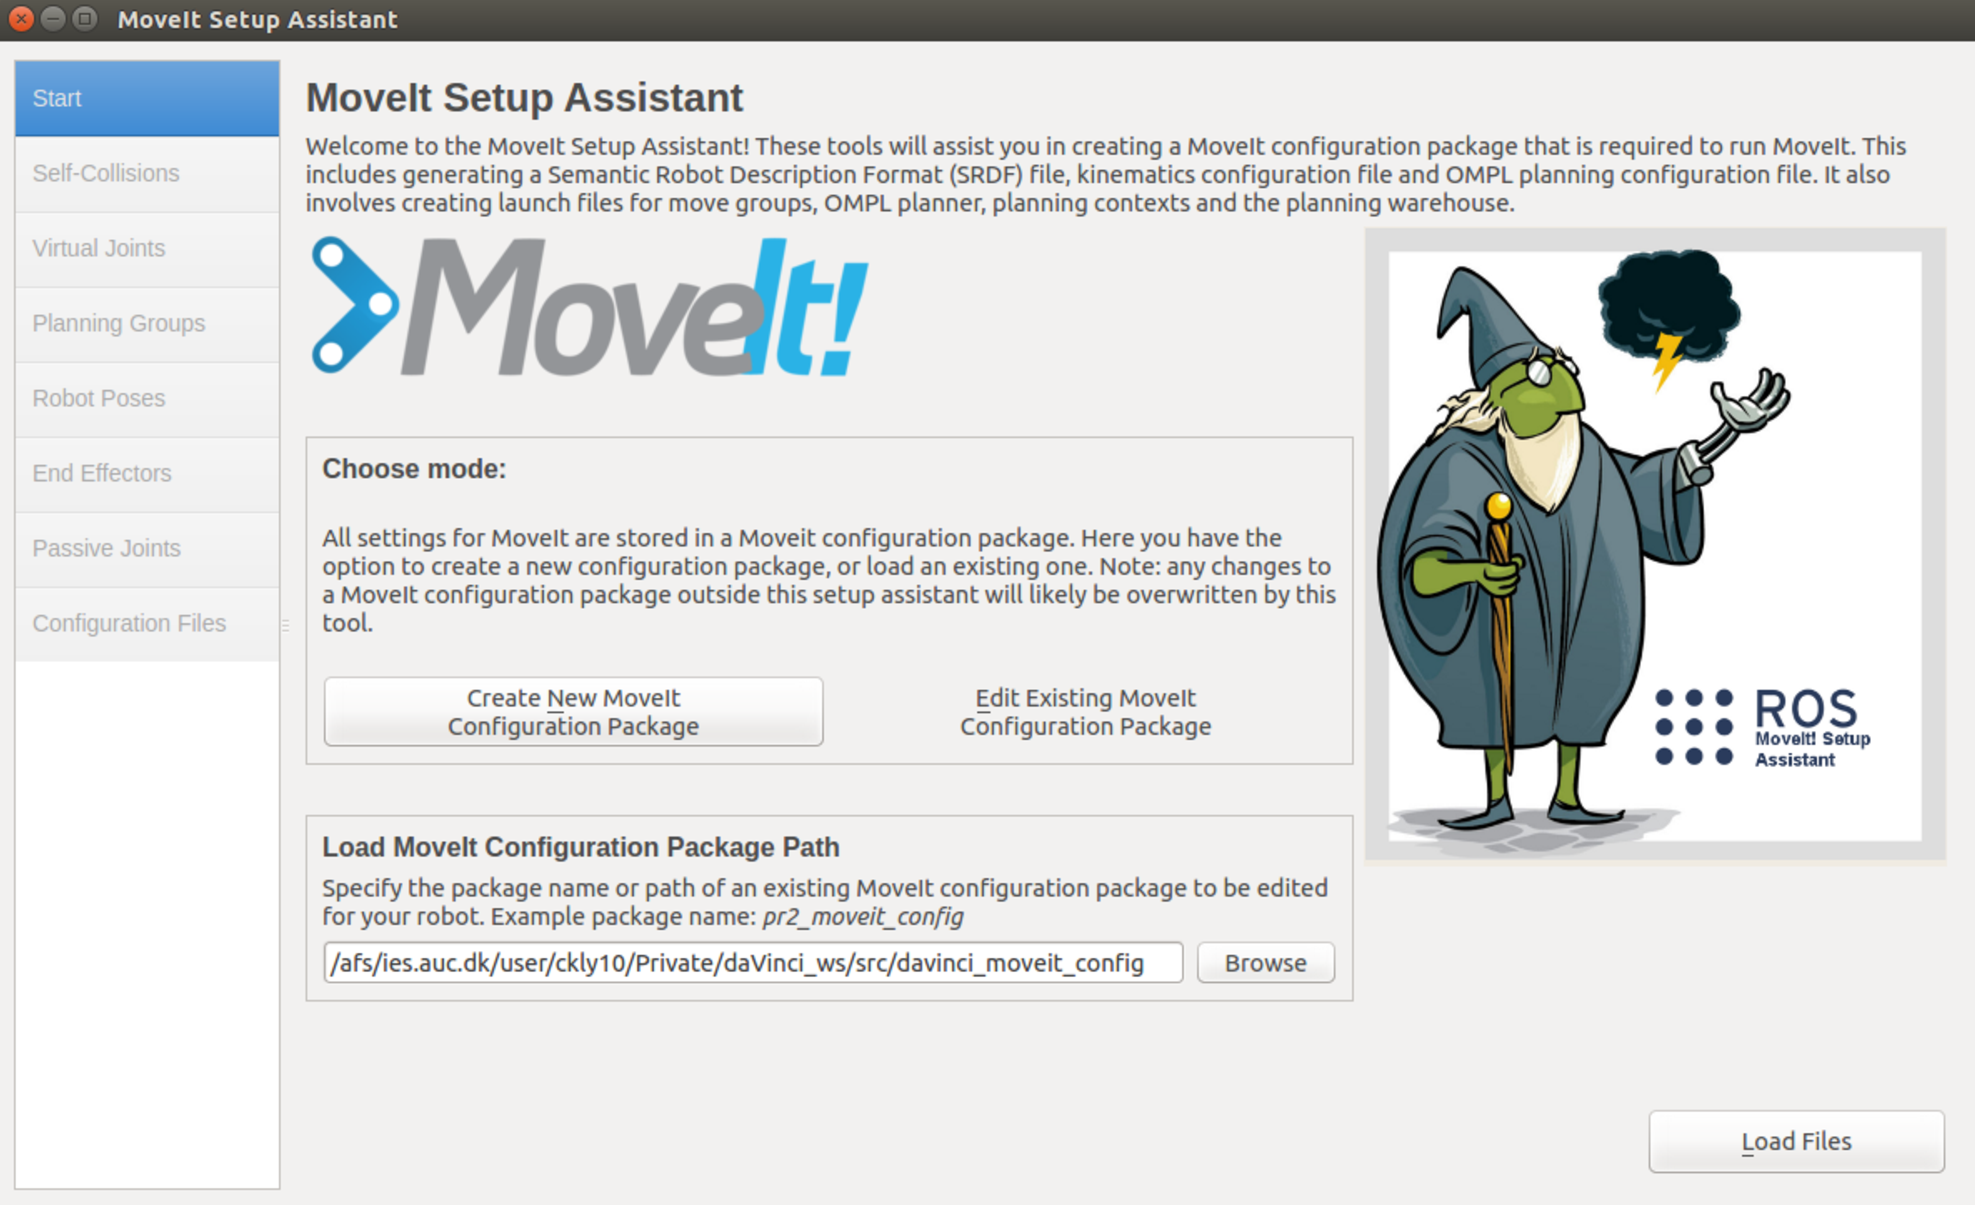
\includegraphics[scale=0.48]{setup_assistant}
%	\caption{Welcome screen by the moveit setup assistant}
%	\label{fig:setup_assistant_init}
%\end{figure}
%\item \textbf{Self Collision:}
This list is auto-generated from the associated xacro files specified in the \texttt{davinci\_} \texttt{description} package (from where a URDF file is generated and initially fed to the setup assistant). The default mode of operation disable collisions between adjacent links, links that can not physically collide, links that are always in collision and links that are in collision in the start-up mode. This ought to enhance processing time \citep{bib:setup_assistant}. It is certainly possible to disable/enable collision between links as needed, though the default operation is used.	
\item \textbf{Virtual Joints:} It is here the robot is attached to the physical world by use of a virtual frame. Make sure the table is filled as shown:
\begin{table}[H]
\hspace{1cm}\begin{tabular}{l|l|l|l}
\textbf{Virtual Joint Name} & \textbf{Child Link}  & \textbf{Parent Frame}  & \textbf{Type}   \\
\hline
 \texttt{virtual\_joint} & \texttt{base\_link}  & \texttt{world}  &  \texttt{fixed} \\
\end{tabular}
\end{table}
\item \textbf{Planning Groups:} It is from here possible to describe the joints of the \texttt{p4\_arm} of da-Vinci. The Orocos \gls{kdl} kinematic solver seems to be dependent of at least six \gls{dof} (six active joints). It is possible to describe the arm by means of either joints, links or as a chain. It is chosen to describe the arm as joints. Be sure that a group \texttt{"gripper"} is added with the following kinematic specifications:
\begin{itemize}
\item Kinematic Solver: \texttt{kdl\_kinematic\_plugin/KDLKinematicPlugin}
\item Kin. Search Resolution: 0.005 (default)
\item Kin. Search Timeout (sec): 0.005 (default)
\item Kin. Solver Attempts: 3 (default)
\end{itemize}
It is furthermore important that it has the following joints specified:
\renewcommand*\DTstylecomment{\rmfamily\color{gray}\textsc}
\renewcommand*\DTstyle{\ttfamily\textcolor{black}} 
\begin{figure}[H]
\dirtree{%
.1 \textbf{\texttt{gripper}}. 
.2 joints.
.3 p4\_instrument\_slide - Prismatic.
.3 p4\_instrument\_roll - Revolute.
.3 p4\_hand\_pitch - Revolute.
.3 p4\_hand\_roll - Revolute.
.3 p4\_rcm\_instrument\_holder\_upper\_bar\_joint - Revolute.
.3 p4\_rcm\_upper\_bar\_base\_joint - Revolute.
.3 p4\_instrument\_jaw\_right - Revolute.
.2 Links \hspace{1cm}\color{gray}{\# Leave this empty}.
.2 Chain \hspace{1cm}\color{gray}{\# Leave this empty}.
.2 Subgroups \hspace{0.2cm}\color{gray}{\# Leave this empty}.
}
\end{figure}
This ensures that the group \texttt{gripper} can operate with six \gls{dof}. It is 
\item \textbf{Robot Poses:} It is from here possible to specify standard positions for the arm. The code developed during this thesis utilized a pose for an initial positions, hence be sure that a pose named \texttt{ready} is present under the group \texttt{gripper}. All joint states should be set to zero for this pose.
\item \textbf{End Effectors:} The end-effector is specified as shown:
\begin{table}[H]
\hspace{1cm}\begin{tabular}{l|l|l|l}
\textbf{End-Effector Name} & \textbf{Group Name}  & \textbf{Parent Link}  & \textbf{Parent Group}   \\
\hline
 \texttt{Gripper} & \texttt{gripper}  & \texttt{base\_link}  &  \texttt{--leave this empty--} \\
\end{tabular}
\end{table}
\item \textbf{Passive Joints:} A list of all joints will be available. It is important to specify the passive joints such that the \texttt{davinci\_moveit\_config} package know which joints are controllable. The table below shows how is must look:
\begin{table}[H]
\hspace{1cm}\begin{tabular}{l|l}
\textbf{Active joints} & \textbf{Passive Joints} \\
\hline
 \texttt{p4\_arm\_elevation} & \texttt{p4\_arm\_elevation} \\
  \texttt{p4\_arm\_yaw1} & \texttt{p4\_arm\_yaw1} \\
   \texttt{p4\_arm\_yaw2} & \texttt{p4\_arm\_yaw2} \\
    \texttt{p4\_arm\_yaw3} & \texttt{p4\_arm\_yaw3} \\
     \texttt{p4\_arm\_roll1} & \texttt{p4\_arm\_roll1} \\
      \texttt{p4\_arm\_yaw4} & \texttt{p4\_arm\_yaw4} \\
       \texttt{p4\_hand\_roll} & \texttt{p4\_rcm\_instrument\_holder\_upper\_bar\_joint} \\
        \texttt{p4\_hand\_pitch} & \texttt{p4\_rcm\_instrument\_bar\_joint} \\
          \texttt{p4\_rcm\_upper\_bar\_base\_joint} &  \\
   \texttt{p4\_rcm\_instrument\_holder\_upper\_bar\_joint} & \\
    \texttt{p4\_instrument\_slide} & \\
     \texttt{p4\_instrument\_roll} &  \\
      \texttt{p4\_instrument\_pitch} & \\
       \texttt{p4\_instrument\_jaw\_left} & \\
        \texttt{p4\_instrument\_jaw\_right} & \\
\end{tabular}
\end{table}
\item \textbf{Configuration Files:} The package will be generated from here by pressing the associated button. It is important to manually check out the files that should be generated. It is important to either recopy the below listed files to the package again or leave them apart from the setup assistant.
\begin{itemize}
	\item \texttt{src/davinci\_moveit\_config/launch/davinci\_moveit\_controller\_manager.launch}
	\item \texttt{src/davinci\_moveit\_config/config/controllers.yaml}
	\item \texttt{CMakeLists.txt}
	\item \texttt{package.xml}
\end{itemize}
It is finally of great significance to modify the \texttt{p4\_hand\_controller.yaml} file in the \texttt{davinci\_driver} package to include the correct joints. This should be taken care of when the development branch is cloned.
\end{enumerate}
%Files that needs to be created/modified manually when the setup assistant is launched:
%
%
\section{Specific Structure of this Thesis - The gr1032 Development Branch}
Be sure that ROS is installed according to the beginning of this appendix. Additionally, the low level controllers and ROS must be initiated as described in \autoref{sec:init_ROS}. The \texttt{gr1032} package can be cloned from github as:

\hspace{0.0cm}  \texttt{git clone https://github.com/AalborgUniversity-RoboticSurgeryGroup/Gr1032}

If the original \texttt{davinci\_description} and \texttt{davinci\_driver} package are cloned to the workspace, delete them. It is important that the \texttt{gr1032} branch is cloned from the driver package and the description package as:

\hspace{0.0cm}  \texttt{git clone https://github.com/AalborgUniversity-RoboticSurgeryGroup/davinci\_driver ---branch gr1032}

\hspace{0.0cm}  \texttt{git clone https://github.com/AalborgUniversity-RoboticSurgeryGroup/davinci\_description ---branch gr1032}

The file structure in the \texttt{daVinci} workspace should be similar to the one depicted below (plus additional files).
\begin{figure}[H]
% to make comment:
% .4 davinci\_moveit\_config\DTcomment{Guillaume}.
\dirtree{%
.1 /...
.2 davinci\_ws. %\DTcomment{workspace folder, created by mkdir}.
.3 \color{ForestGreen}{run\_controllers.py} \color{gray}{wrapper script}.
.3 build. %\DTcomment{generated by catkin\_init\_workspace}.
%.4 \color{gray}{..}.
.4 \color{gray}{... all make-files}. %\DTcomment{generated by catkin\_init\_workspace}.
.3 devel. %\DTcomment{generated by catkin\_init\_workspace}.
%.4 \color{gray}{..}.
.4 \color{gray}{... all libraries and setup files}. %\DTcomment{generated by catkin\_init\_workspace}.
.3 src.
.4 \color{ForestGreen}{CMakeLists.txt}.
.4 davinci\_description. %\DTcomment{\underline{Package:} Physical sizes and rotation matrices}.
.5 \color{ForestGreen}{CMakeLists.txt}.
.5 config.
.6 \color{ForestGreen}{davinci.rviz}.
.5 launch.
.6 \color{ForestGreen}{demo.launch}.
.6 \color{ForestGreen}{visualize\_in\_rviz.launch}.
.5 meshes.
.6 \color{gray}{... all .stl files (used for the 3D model in rviz)}.
.5 \color{ForestGreen}{package.xml}.
.5 robots.
.6 \color{ForestGreen}{remote\_center\_manipulator.xacro}\hspace{0.2cm}\color{gray}{\# rotation matrices for the hand}.
.6 \color{ForestGreen}{davinci.xacro}\hspace{0.2cm}\color{gray}{\# assembles all xml macros}.
.6 \color{ForestGreen}{p4\_arm.xacro}\hspace{0.2cm}\color{gray}{\# rotation matrices for the arm}.
.6 instruments.
.7 \color{ForestGreen}{needle\_driver.xacro}\hspace{0.2cm}\color{gray}{\# rotation matrices for instrument}.
.4 davinci\_driver. %\DTcomment{\underline{Package:} Interface with the physical robot}.
.5 \color{ForestGreen}{CMakeLists.txt}.
.5 launch.
.6 \color{ForestGreen}{davinci\_driver.launch} \color{gray}{\# include control output}.
.6 \color{ForestGreen}{ros\_control.launch} \color{gray}{\# include controllers}.
.5 src.  
.6 \color{ForestGreen}{davinci\_driver.cpp}\hspace{0.2cm}\color{gray}{\# establish connection }.
.6 \color{ForestGreen}{ros\_driver.cpp}\hspace{0.2cm}\color{gray}{\# establish connection }.
.6 \color{ForestGreen}{sbrio\_driver.cpp}\hspace{0.2cm}\color{gray}{\# establish connection }.
.5 config.
.6 \color{ForestGreen}{davinci\_ip\_adresses.yaml}\hspace{0.2cm}\color{gray}{\# set IP for RIO primary/secondary board}.
.6 \color{ForestGreen}{p4\_hand\_controller.yaml}\hspace{0.2cm}\color{gray}{\# specify each controllable joint}.
.4 gr1032.
.5 \color{ForestGreen}{CMakeLists.txt}.
.5 \color{ForestGreen}{package.xml}.
.5 src.
.6 \color{ForestGreen}{run\_controller.cpp} \color{gray}{\# main C++ interface (controllers) }.
.5 launch \color{gray}{\# not used}.
}
\end{figure}
The controllers are executed by running the two commands below in two individual terminals:
\begin{itemize}
\item \texttt{roslaunch davinci\_driver davinci\_driver.launch}
\item \texttt{python run\_controllers.py}
\end{itemize}
This leaves a \gls{gui} as shown below:
\lstdefinestyle{DOS}
{
    backgroundcolor=\color{white},
    basicstyle=\scriptsize\color{black}\ttfamily
}
\begin{lstlisting}[style=DOS]
*******************************************
The following options are avaiable:
-------------------------------------------
press 'a' to run slide safety controller
press 'b' to run custom joint angles
press 'c' to run demo:
press 'd' to run beating heart controller:
*******************************************
\end{lstlisting}
The desired controller is now ready to be executed by entering the inquired letters. The \texttt{gr1032} package provides also demo's which the exclusive purpose of demonstrating the capabilities of the Da Vinci robot. The file and code structure is not as such described deeper in this appendix. The algorithms associated with each controller is described under each appertaining chapter in the main report. 
\subsubsection*{Useful and Regularly used ROS Commands}
To build the entire environment, navigate to the root of the workspace and type:

\hspace{1cm} \textbf{$\bullet$} \ \ \  \texttt{\$ catkin\_make}% \ \ \ {\color{RoyalBlue}{\textit{\# read various state information from terminal output}}} 

The current joint position is per default broadcasted to the topic \texttt{joint\_states}. To subscribe to this topic, open a terminal and type:

\hspace{1cm} \textbf{$\bullet$} \ \ \  \texttt{\$ rostopic echo joint\_states} \ \ \ {\color{RoyalBlue}{\textit{\# read all state information from terminal output}}} 

\hspace{1cm} \textbf{$\bullet$} \ \ \  \texttt{\$ rostopic echo joint\_states/position[$n$]} \ \ \  {\color{RoyalBlue}{\textit{\# read the $n^\text{th}$ joint state}}} 

Obtain a list of the used kinematic solvers, open a terminal and type:

\hspace{1cm} \textbf{$\bullet$} \ \ \  \texttt{\$ rosparam list | grep kinematics} \ \ \ {\color{RoyalBlue}{\textit{\# read solvers from terminal}}} 

view to all active topics:

\hspace{1cm} \textbf{$\bullet$} \ \ \  \texttt{\$ rostopic list} \ \ \ {\color{RoyalBlue}{\textit{\# read topics from terminal}}} 

Similar, see all active nodes as: 

\hspace{1cm} \textbf{$\bullet$} \ \ \  \texttt{\$ rosnode list} \ \ \ {\color{RoyalBlue}{\textit{\# read nodes from terminal}}} 

To create a \gls{urdf} file from the present xacro files, type the below command from the root of the workspace:

\hspace{1cm} \textbf{$\bullet$} \ \ \  \texttt{\$ rosrun xacro xacro.py src/davinci\_description/robots/davinci.xacro > <name>.URDF} %\ \ \ {\color{RoyalBlue}{\textit{\# URDF is created}}} 
%
\subsection*{Useful Debugging Commands}
To check which files are recently modified, open a terminal and run:

\hspace{1cm} \textbf{$\bullet$} \ \ \  \texttt{\$ find . -type f -exec ls -lt $\backslash$\{$\backslash$\} $\backslash$+ | head} 

This is fairly useful as, for example, the setup-assistant overwrites a number of files. 

{\color{white}{\gls{yaml}}}{\color{white}{\gls{xacro}}}